\documentclass[a4paper,12pt]{article}
\usepackage{graphicx} 
\usepackage[polish]{babel}
\usepackage[OT4]{fontenc}
\usepackage[utf8]{inputenc}
\author{Krzysztof Rokicki}
\title{Sprawozdanie ze sprawdzianu}
\date{\today}
\begin{document}
\maketitle
\section{Zad 1}
Najpierw aby stworzyć klucze użyłem komendy ssh-keygen. Potem musiałem wybrać miejsce w którym ma się ten klucz zapisać  podać hasło dostępu do niego.\\
\begin{figure}
\centering
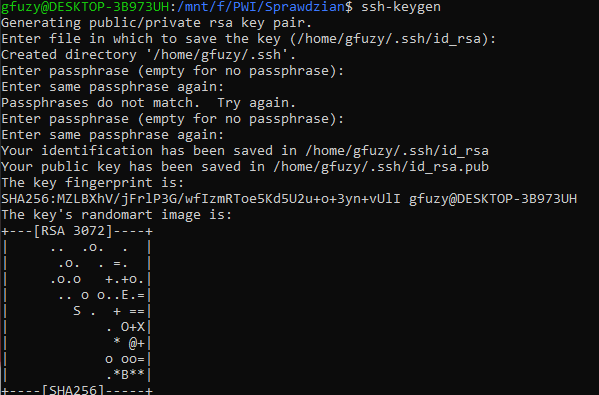
\includegraphics[width=10cm]{ssh-keygen}
\caption{Użycie komendy ssh-keygen}
\end{figure}
Następnie mieliśmy dodać klucz na serwer. Zrobiłem to używając komendy:
\begin{center}
 ssh-copy-id (adres klucza) mpyzik@pwi.ii.uni.wroc.pl
\end{center}
Po czym trzeba było jeszcze wpisać hasło.
\begin{figure}
\centering
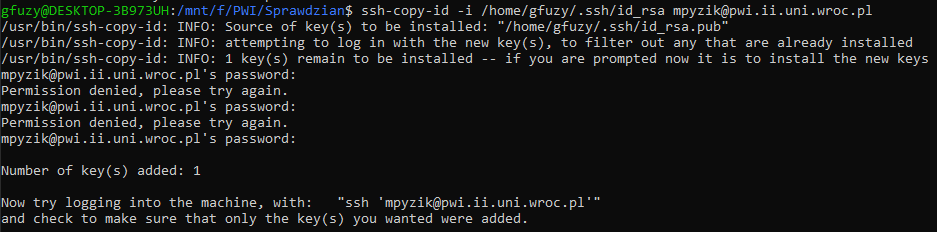
\includegraphics[width=15cm]{ssh-copy-id}
\caption{Użycie komendy ssh-copy-id}
\end{figure}
Ostatnim krokiem było wejście na serwer, do którego użyłem danej komendy:
\begin{center}
 ssh mpyzik@pwi.ii.uni.wroc.pl
\end{center}
Dzięki temu, że wgrałem wcześniej klucz na serwer nie musiałem podawać hasła konta, tylko musiałem podać hasło które przypisałem do klucza.
\begin{figure}
\centering
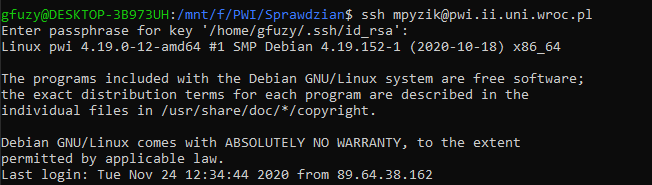
\includegraphics[width=10cm]{ssh}
\caption{Użycie komendy ssh}
\end{figure}
\section{Zad 2}
W tym zadaniu mieliśmy stworzyc plik z naszą nazwą i wpisać w nim swoje imię i nazwisko oraz numer indeksu. Plik stworzyłem komendą touch, a plik edytowałem dzięki edytorowi nano.\\
Aby dodać datę użyłem komendy echo, która wyglądała tak:
\begin{center}
echo `date` >> krzysztof\_rokicki
\end{center}
Aby dodać ciąg liczby podzielnych przez 7 użyłem takiej komendy:
\begin{center}
echo `seq 7 7 100` >> krzysztof\_rokicki
\end{center} 
Ostatnim krokiem było pobranie naszego pliku. W tym celu najpierw stworzyłem folder testy komendą mkdir i przenioslem tam plik komendą mv. Na koniec wyszedłem z serwera i będąc na swoim dysku zastosowałem komendę:
\begin{center}
scp mpyzik@pwi.ii.uni.wroc.pl:$\sim$/testy/krzysztof\_rokicki krzysztof\_rokicki
\end{center}
\end{document}